\section{Multigroup Approximation}\label{apxMultigroup}

In many transport problems, the cross section or opacity of a material is not
simply described by a continuous function.  At many different energies (or
frequencies), radically different characteristics may be found for absorption
or scattering of incident radiation.  A ``multigroup approximation'' is often
performed, which allows the chief characteristics of individual energy spectra
to be represented as a sum instead of a continuous integral.  Without making
any approximation, the integrated value of a general function $f(\nu)$ can be
represented as
\[\int_0^\infty f(\nu)\ d\nu = \sum_{\nu=0}^\infty f(\nu).\]

Furthermore, we can split this continuous sum into groups of continuous sums,
still without making any approximations:
\[\int_0^\infty f(\nu)\ d\nu = \sum_{g=0}^\infty f_g,\]
where the group function is defined
\[f_g\equiv\int_g^{g-1} f(\nu)\ d\nu.\]
Note here that lower values of $g$ correspond to higher values of $\nu$.  While
this may be somewhat confusing, it is the typical convention in multigroup
theory.

Since finding the integrated value of $f(\nu)$ is still no easier than before,
we now make an approximation by truncating the infinite sum:
\[\int_0^\infty f(\nu)\ d\nu \approx \sum_{g=0}^G f_g.\]
In the limit that $G\to\infty$, there is no approximation made.

As necessary, further approximation can be made if $f(\nu)$ is separable into
several functions of $\nu$.  For example, let
\[f(\nu) = \frac{A(\nu)B(\nu)}{C(\nu)}.\]
In the multigroup approximation, then,
\[\int_0^\infty f(\nu) \approx \sum_{g=0}^G f_g
   = \sum_{g=0}^G \frac{A_gB_g}{C_g}.\]
This is an approximation in that, for the general case,
\[\int \frac{A(x)B(x)}{C(x)}\ dx
   \neq \frac{\int A(x)\ dx\ \int B(x)\ dx}{\int C(x)\ dx}.\]
However, using these multigroup approximations, previously-inhibiting
integrations can be discretized into terms that can be computed.

\subsection{Riemann Approximation}
In this work, a Riemann approximation is used to find the group values for
continuous integrals as described above.  The basic tenet of this approximation
is that continuous integrals may be approximated as the sum of many trapezoidal
figures that roughly approximate the shape of the integrand (see Figure\
\ref{RiemannFig}).  There are several different methods of implementing the
Riemann sum.  The value of the function over a range can be the function
evaluated at the leftmost part of the range, the value at the rightmost part
of the range, or the value in the center of the range.  The approximation in
Figure\ \ref{RiemannFig} is representative of a fourth, more
accurate method: the ``trapezoidal'' method.  In this method, the Riemann
segment an upper value that is the linear-fit average of the function in the
cell instead of the function evaluated at any one point. For this method, the
integral of the function is approximated as
\[\int_a^b f(x)\ dx \approx \sum_{r=1}^R \frac{\big[f(x_r)+f(x_{r+1})\big]
  \Delta r}{2}\]
where $x_r$ is the value of $x$ at the leftmost bound of the Riemann segment.
\begin{figure}[htb]
\centering
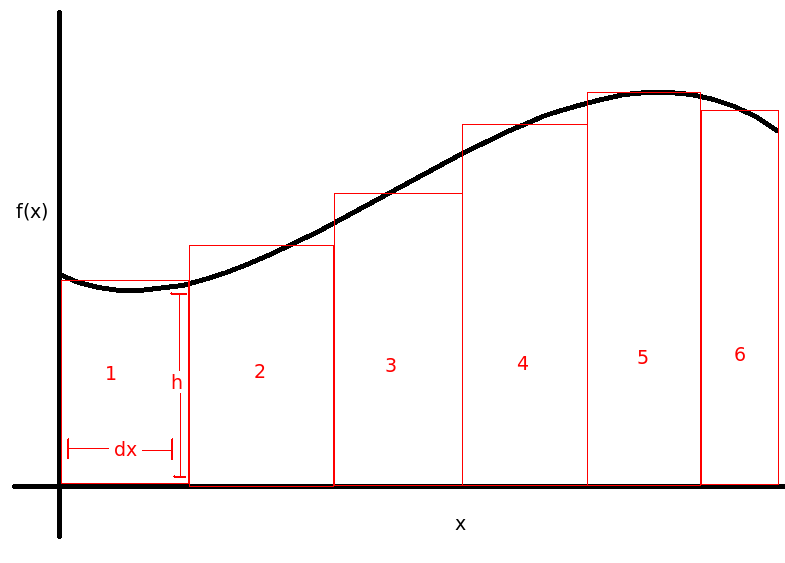
\includegraphics[width=0.7\linewidth]{RiemannFig}
\caption{Visualization of Riemann Sum Method}
\label{RiemannFig}
\end{figure}

\newpage
\subsection{Accuracy of Multigroup Approximation}
In order to compare the multigroup approximation to a more analytic solution,
the DMP was calculated using the multigroup method described above, then with
an analytic solve using the \texttt{MatLab} computer algebra
software. The results are shown in Figure
\ref{mg_vs_anl}. Calculating the relative error between the two methods led to a
machine-precision difference in all cases.  For the large set of runs used to
create the discrete maximum curve shown in Figure \ref{mg_vs_anl}, the analytic
method took about 160 seconds, while the multigroup method took just over 23
seconds, suggesting the multigroup method is on the order of seven times faster
to calculate than the analytic method.
\begin{figure}[htb]
\centering
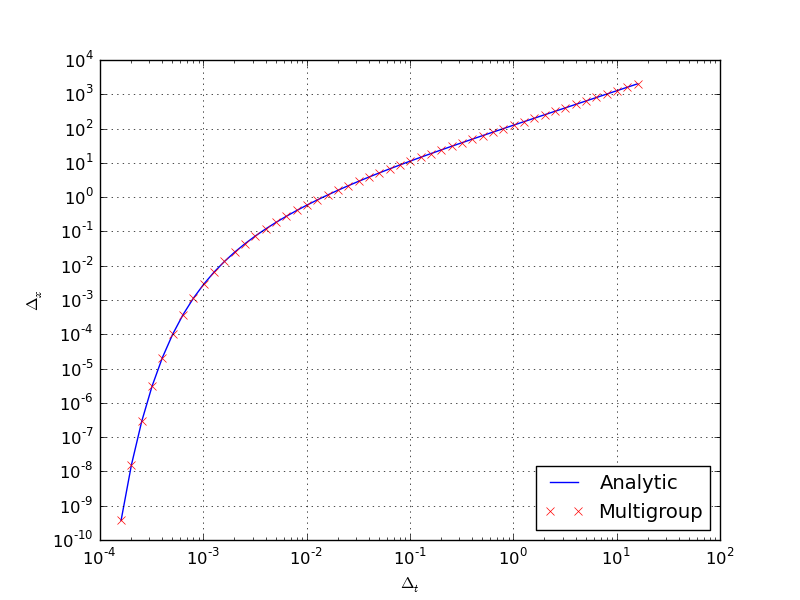
\includegraphics[width=0.7\linewidth]{DMP_mg_numR}
\caption{Multigroup versus Analytic Solutions for the DMP}
\label{mg_vs_anl}
\end{figure}